\documentclass[11pt,a4paper]{article}
\usepackage[utf8]{inputenc}
%\usepackage[brazilian]{babel}
\usepackage{booktabs}
\usepackage{array}
\usepackage{float}
\usepackage{graphicx}
\usepackage{multirow}
\usepackage{enumitem}
\usepackage[a4paper,top=2cm,bottom=1.8cm,left=2.5cm,right=2.5cm,marginparwidth=1.75cm]{geometry}


\begin{document}
\begin{table}[t]
  \centering
  \begin{tabular*}{\textwidth}{p{1.9cm} l@{\extracolsep{\fill}} r}
  \multirow{3}{1.9cm}{{
\includegraphics[width=1.9cm]{positivo_cor.pdf}}}
    & \small{Universidade de Brasília} & \\
	& \small{Faculdade de Tecnologia} & \\
    & Departamento de Engenharia Elétrica & \\
    \midrule
    \multicolumn{2}{l}{ \large ENE337293 - Aprendizado de Máquina} & {\large 2020/2}\\
    \multicolumn{2}{l}{Prof.  Daniel Guerreiro e Silva} & \\
    \multicolumn{2}{l}{Aluno: Guilherme Fay Vergara} & Matr.: 20/0097458 \\
  \end{tabular*}
\end{table}

\begin{center}
{\LARGE \bf Assignment 1}
\end{center}

\section{}
\begin{enumerate}[label=(\alph*)]
\item \parbox{\linewidth}

\begin{figure}[ht!]
    \centering
    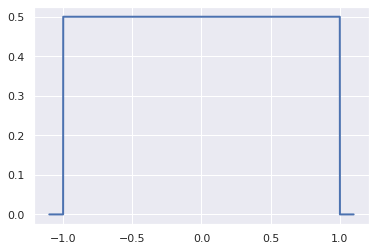
\includegraphics{figuras/1a.png}
    \caption{Probability density function}
    \label{fig:1a}
\end{figure}

The area is given by the area of rectangle $B*H$  where the base is $2$ and the height is $0.5 = 2*0.5 = \textbf{1}$

\item \parbox{\linewidth}

\begin{figure}[ht!]
    \centering
    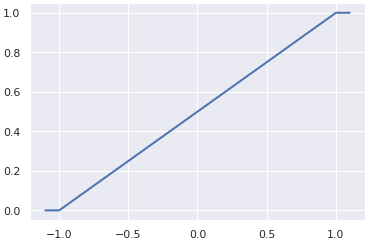
\includegraphics{figuras/1b.png}
    \caption{Probability density function}
    \label{fig:1a}
\end{figure}

\item The probability is given by the area $B*H$ where the base is $0.4$ and the height is $0.5 = 0.4*0.5 = 0.2 = \textbf{20\%}$

\item The expected value is calculated by

\begin{equation}
E(X^{n}) = \frac{1}{n+1} \sum_{k=0}^{n} a^{k}b^{n-k}
\end{equation}

\begin{itemize}
    \item\textbf{$E(X)$}
    \\
    \\
    $E(X) = \frac{1}{2} (1+1) = \textbf{1}$
    \\
    
    \item\textbf{$E(X^{2})$} 
    \\
    \\
    $E(X^{2}) = \frac{1^{3} - (-1)^{3}}{3*1-3*(-1)}$
    \\
    \\
    $E(X^{2}) = \frac{2}{6} = \frac{1}{3} = \textbf{0.333...}$
    \\
    
    \item\textbf{$E(X^{4})$}
    \\
    \\
    $E(X^{4}) = \frac{1^{5} - (-1)^{5}}{5*1-5*(-1)}$
    \\
    \\
    $E(X^{4}) = \frac{2}{10} = \frac{1}{5} = \textbf{0.2}$
    \\
    
    \item\textbf{$VarE(X)$}
    The variance is calculated by

    \begin{equation}
       V(X) = \frac{1}{12} (b-a)^{2}
    \end{equation}
    \\
    \\
   By (2) we have $V(X) = \frac{4}{12} = \frac{1}{3} = \textbf{0.333...}$
    
\end{itemize}






\end{enumerate}



\section{}


\section{}




%\bibliographystyle{plain}
%\bibliography{epistem}

\end{document}
